\documentclass[a4paper,10pt]{jsarticle}

% レイアウト
\setlength{\textwidth}{\fullwidth}
\setlength{\textheight}{39\baselineskip}
\addtolength{\textheight}{\topskip}
\setlength{\voffset}{-0.5in}
\setlength{\headsep}{0.3in}
\pagestyle{myheadings}

% パッケージ
\usepackage[dvipdfmx]{graphicx}
\usepackage{amsmath,amssymb,epsfig}
\usepackage{bm}
\usepackage{ascmac}
\usepackage{pifont}
\usepackage{multirow}
\usepackage{enumerate}
\usepackage{cases}
\usepackage{type1cm}
\usepackage{cancel}
\usepackage{url}
\usepackage{color}
\usepackage{listings,jlisting}
% 大きな中括弧
\usepackage{cases}

% 定義
\DeclareMathOperator*{\argmin}{arg\,min}
\DeclareMathOperator*{\argmax}{arg\,max}
\def\vec#1{\mbox{\boldmath$#1$}}
\def\R{{\Bbb R}}

% カウンタの設定
\setcounter{section}{0}
\setcounter{subsection}{0}
\setcounter{subsubsection}{0}
\setcounter{equation}{0}

% キャプションの図をFigに変更
\renewcommand{\figurename}{Fig.}
\renewcommand{\tablename}{Tab.}

% 式番号を式(章番号.番号)に
% \makeatletter
% \renewcommand{\theequation}{\arabic{section}.\arabic{equation}}
% \@addtoreset{equation}{section}
% \makeatother

% プログラムに色をつける
\usepackage{color}

\definecolor{codegreen}{rgb}{0,0.6,0}
\definecolor{codegray}{rgb}{0.5,0.5,0.5}
\definecolor{codepurple}{rgb}{0.58,0,0.82}
\definecolor{backcolour}{rgb}{0.95,0.95,0.92}

\lstdefinestyle{mystyle}{
    backgroundcolor=\color{backcolour},
    commentstyle=\color{codegreen},
    keywordstyle=\color{magenta},
    numberstyle=\tiny\color{codegray},
    stringstyle=\color{codepurple},
    basicstyle=\footnotesize,
    breakatwhitespace=false,
    breaklines=true,
    captionpos=b,
    keepspaces=true,
    numbers=left,
    numbersep=5pt,
    showspaces=false,
    showstringspaces=false,
    showtabs=false,
    tabsize=2
}

\lstset{style=mystyle}

% 表紙
\title{知能システム学特論レポート}
\author{
(DL2班)Caffe on Ubuntu\\
}
\date{2015年\ 7月\ 16日}

% ドキュメントの開始
\begin{document}
\maketitle
\section{報告者}
\begin{list}{}{}
 \item 15344203\hspace{0.5cm} 有田 裕太
 \item 15344206\hspace{0.5cm} 緒形 裕太
 \item 15344209\hspace{0.5cm} 株丹 亮
 \item 12104125\hspace{0.5cm} 宮本 和
\end{list}

\section{進行状況}

\begin{itemize}
\item 畳み込みネットワークと正規化層の理論について
\item データセットの作成準備
\end{itemize}

\section{理論研究}
\subsection{勾配の計算}
畳み込み層の計算式は,順伝播型ニューラルネットワークの中間層と同様に次のように表すことができる.
\begin{equation}
 u^{(l)} = W^{(l)} u^{(l-1)} + b^{(l)}
\end{equation}
\begin{equation}
 z^{(l)} = f^{(l)} (u)
\end{equation}

ただし$W$は,サイズ$H\times H\times K$の$M$個のフィルタの係数$h_{pqkm}$を畳み込みを再現するように規則的に並べたものである.
逆伝播の計算も全結合層の場合と基本的には同じだが,$W^{(l)}$に同じフィルタの係数が何度も現れることを考慮する必要がある.これを表現するために,フィルタの係数$h_{pqkm}$から行列$W = W^{(l)}$を作る過程を以下に示す.まず,フィルタの係数を適当な順で並べ,成分数$H\times H\times K\times M$のベクトル$h$を作る.次に$h$と同じ長さを持ち$h$との内積が,重み$w_{ji}$を与えるベクトルを$t_{ji}$と定義する.
\begin{equation}
 W_{ji} = t_{ji}^{T} h
\end{equation}

そして$t_{ji}$の成分を$t_{jir}$と書き,$r$を固定したとき$t_{jir}$を$(j,i)$成分にもつ行列を$T_r$と書く.

%%%%%% ogata %%%%%%
\subsection{誤差関数}
本班のcaffeを用いた画像分類では,第4回レポートで記したような多クラス分
類を行っており,出力関数はソフトマックス関数である.多クラス分類ではネッ
トワークが実現する関数を各クラスの事後確率のモデルであると見なし,そのモ
デルのもとで訓練データに対するネットワークパラメータの尤度を評価し,これ
を最大化する.いま訓練データとして,入力${\bf x}$とその正解クラスの組$C_k$が与え
られたとする.このときの目標出力を2値の値を$K$個並べたベクトル${\bf
d}_n$によって表現すると,事後分布は次式のようになる.

\begin{equation}
 p({\bf d}|{\bf x}) = \prod_{k=1}^{K}p(C_k|{\bf x})^{d_k}
\end{equation}

これより,訓練データ${({\bf x}_n|{\bf d}_n)}(n=1,...,N)$に対する{\bf w}
の尤度は

\begin{equation}
 L({\bf w})=\prod_{n=1}^{N}p({\bf x}_n|{\bf x}_n;{\bf
	w})=\prod_{n=1}^{N}\prod_{k=1}^{K}p(C_k|{\bf
	x})^{d_{nk}}=\prod_{n=1}^{N}\prod_{k=1}^{K}(y_k({\bf x};{\bf w}))^{d_{nk}}
\end{equation}

と導ける.この尤度の対数とって符号を反転した次の式を誤差関数として用いる.
この関数は交差エントロピー(cross entropy)と呼ばれる.
\begin{eqnarray}
 E({\bf w})=-\sum^{N}_{n=1}\sum^{N}_{k=1}d_{nk}\log
	y_{k}(\vec{x}_{n};{\bf w})\label{000700_27Jun15}
\end{eqnarray}


\section{プログラミング}
\subsection{学習パラメータの設定}
学習を行う上で必要なパラメータについて説明する.この設定が記述されているファイルはcifar10\_quick\_solver.prototxtである.
以下に設定ファイルの内容を示し,各パラメータに関する意味を記述する.

\begin{lstlisting}[basicstyle=\ttfamily\footnotesize, frame=single, firstnumber=1, numbers=left, breaklines=true]
net: "examples/cifar10/cifar10_quick_train_test.prototxt"
test_iter: 100
test_interval: 500
base_lr: 0.0001
momentum: 0.9
weight_decay: 0.004
lr_policy: "fixed"
display: 100
max_iter: 4000
snapshot: 4000
snapshot_prefix: "examples/cifar10/cifar10_quick"
solver_mode: GPU
\end{lstlisting}

ここでバッチ数と呼ばれる単位を導入する.バッチ数は教師データを一度にいくつ処理するか(バッチサイズ)を決定し,これを1[batch]とする.
Caffeでは繰り返し数をバッチ数で指定している.

\begin{description}
  \item[net :]学習用ネットワーク定義ファイルを指定する.
  \item[test\_iter :]学習中の正答率評価を1回行うのに使う評価セットのデータ数をバッチ数で指定.評価セットのデータ数とバッチサイズの除算を行い,この数値を設定することで正答率評価にすべての評価セットを用いることができる.
  \item[test\_interval :]テストデータから正答率評価を行う間隔をバッチ数で指定.データ数が多い場合,正答評価に多くの時間がかかるので用いるデータセットの規模によって適切な値に設定する必要がある.
  \item[base\_lr,\ momentum,\ weight\_decay,\ lr\_policy :]学習率に関する設定.
  \item[display :]学習中のステータスを出力する回数をバッチ数で指定.
  \item[max\_iter :]学習の計算を最大どれだけ続けるかを訓練データのバッチ数で指定.ここで指定された数値とバッチサイズの積算が学習が終了するまでの処理する画像枚数となる.
  \item[snapshot,\ snapshot\_prefix :]学習の途中経過を保存する間隔と場所を指定.
  \item[solver\_mode :]学習をCPUのみ,あるいはGPUを用いるかを指定.
\end{description}

\subsection{訓練データの作成}
独自の訓練データを用いて学習を行うということで今回はアニメ「ラブライブ!」における主要キャラクターの識別をDeep Learningで行うことを目標とした.そこで,まず訓練データを作成した.訓練データはキャラクター毎に約2000枚程度集めた.これはアニメの中からHaar-like特徴量を用いて顔検出を行い,その顔検出によって得られた矩形を切り出し保存したものを人間の目によって分類して集めた.また,キャラクターの顔画像の他に負例として7000枚ほど当該キャラクター以外の顔画像やそもそも顔画像ではない画像も集めている.以上の訓練データの画像は全て$200\times200$にリサイズを行っている.


その後,前回の説明であった通り,$1:9$の割合でテストデータと訓練データにランダムに分け,caffeで用いられるデータ形式に変換後,学習を実行する.

\subsection{学習}
学習は以下のコマンドで実行される.

\begin{lstlisting}[basicstyle=\ttfamily\footnotesize, frame=single, tabsize=2,showtabs,firstnumber=1, numbers=left, breaklines=true]
build/tools/caffe train --solver examples/cifar10/cifar10_quick_solver.prototxt
\end{lstlisting}

今回,アニメキャラクターの顔認識を行うにあたり,ネットワークモデルとしてcifar10のモデルを用いて学習を行った.cifar10のモデルは畳込み層が3層,プーリング層が3層,全結合層が2層からなるCNNであり,活性化関数にはSoftmax関数を用いている.

また,学習を行った際のパラメータの一部を以下に示す.
\begin{itemize}
 \item test\_iter : 100
 \item max\_iter : 4000
 \item batch\_size : 100
 \item solver\_mode : CPU
\end{itemize}

\subsection{学習結果}
学習を行った結果得られた,トレーニングの繰り返し回数と損失関数の値及びテストデータにおける精度のグラフをFig.\ref{210045_15Jul15}に示す.
精度は500イテレートあたりで急激に上昇し,最終的に94.2\%の精度となった.

\begin{figure}[ht]
 \centering
 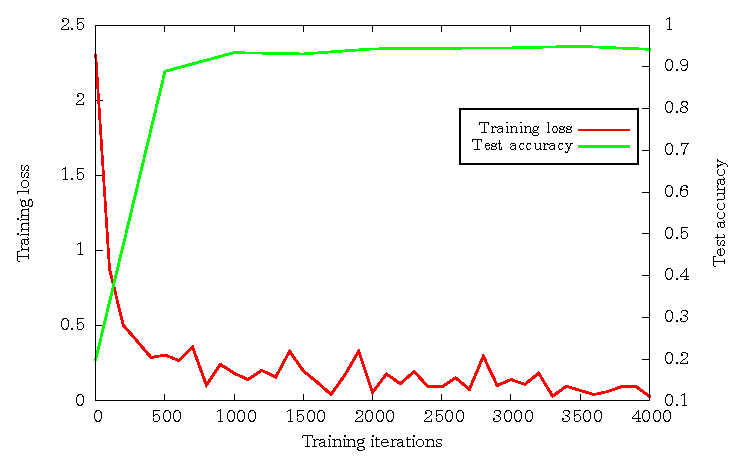
\includegraphics[scale=1.0]{fig/eps/result_train_test_graph.eps}
 \caption{損失関数の値と精度 }
 \label{210045_15Jul15}
\end{figure}

\section{今後の課題}
\begin{itemize}
 \item 理論研究を進める.
 \item データセットの作成,学習実行結果の評価と過程の可視化.
\end{itemize}

\end{document}